\begin{frame}
	\centering
	\begin{figure}[H]
		\includegraphics[keepaspectratio, width=0.7\paperwidth, height=\paperheight]{\thelogo}
	\end{figure}
	Informatik: Programmieren\\
	Weitere Möglichkeiten mit der Turtle\emoji{turtle}:\\
	Farben, Koordinatengrafik, Zufallszahlen
\end{frame}

\begin{frame}[fragile]{Sterne zeichnen \faStar}
	\begin{lstlisting}[numbers=none,style=python]
import turtle as t

def star():
    for _ in range(6):
        t.forward(30)
        t.right(140)
        t.forward(30)
        t.left(80)

star()
\end{lstlisting}
\end{frame}

\begin{frame}[fragile]{\textcolor{ForestGreen}{Neue Farben \faStar}}
	\begin{lstlisting}[numbers=none,style=python]
import turtle as t

def star():
    for _ in range(6):
        t.forward(30)
        t.right(140)
        t.forward(30)
        t.left(80)

t.color(0,155,85)        
star()
\end{lstlisting}
	\lstinline[numbers=none,style=python]|setPenColor(...)|:
	\begin{itemize}
		\item Vordefinierte Farbe auf Englisch, z.B. \lstinline[numbers=none,style=python]|t.color("green")|, \textit{mit} Anführungszeichen
		\item \textcolor{red}{R}\textcolor{green}{G}\textcolor{blue}{B}-Code, z.B. \texttt{t.color(\textcolor{red}{0},\textcolor{green}{155},\textcolor{blue}{85})}, \textit{ohne} Anführungszeichen
	\end{itemize}
\end{frame}

\begin{frame}[fragile]{Reminder: Farben kodieren}
	\begin{figure}[H]
		\centering
		\begin{subfigure}{.49\textwidth}
			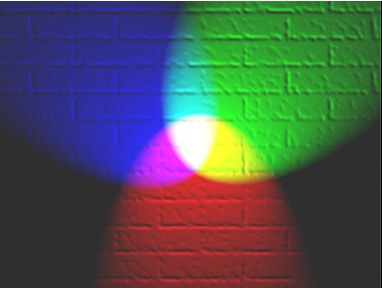
\includegraphics[width=\textwidth]{Grundlagen_Info/01_TheoretischeInformatik/Figures/rgb-farbmischung-1}
		\end{subfigure}
		\begin{subfigure}{.49\textwidth}
			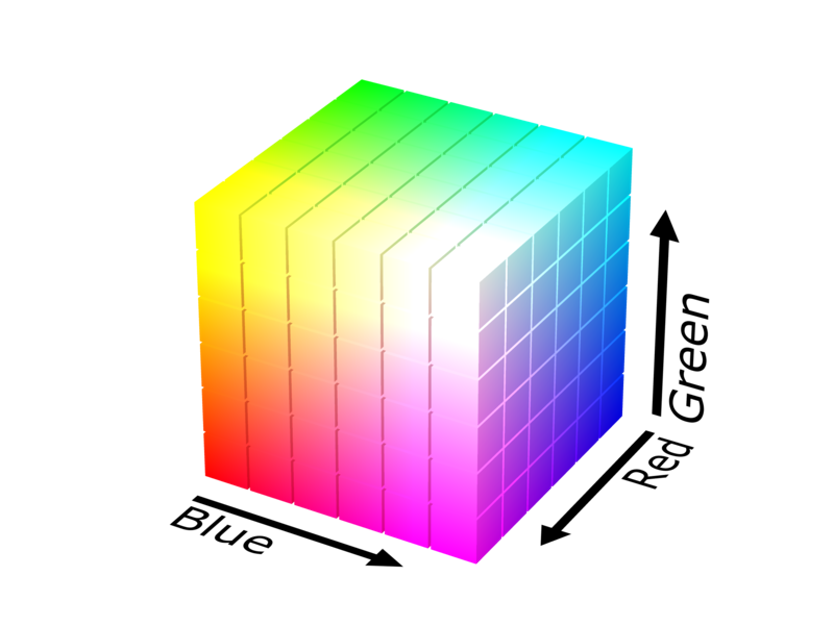
\includegraphics[width=\textwidth]{Grundlagen_Info/01_TheoretischeInformatik/Figures/rgb-farbmischung-2}
		\end{subfigure}
	\end{figure}
	$\rightarrow$ Jede Farbe kodiert zwischen 0 und 255!
	\only<2->{
		\red{11111111}\green{00000000}\blue{00000000} = \#\red{FF}\green{00}\blue{00} = \red{255}\green{0}\blue{0} = reines Rot\\

		\red{10000000}\green{10000000}\blue{10000000} = \#\red{80}\green{80}\blue{80} = \red{128}\green{128}\blue{128} = grau}
\end{frame}

\begin{frame}[fragile]{\lstinline[style=python]|clear(farbe)|}
	\begin{lstlisting}[style=python]
import turtle as tabwin

def star():
    for _ in range(6):
        t.forward(30)
        t.right(140)
        t.forward(30)
        t.left(80)

t.clear("blue")
star()
\end{lstlisting}
	\begin{itemize}
		\item \lstinline[numbers=none,style=python]|t.clear(...)|: Hintergrund auf bestimmte Farbe setzen (Name oder RGB-Code)
	\end{itemize}
\end{frame}

\begin{frame}[fragile]{Flächen ausfüllen mit \lstinline[numbers=none,style=python]|fillPath()|}
	\begin{lstlisting}[numbers=none,style=python]
import turtle as t

def star():
    for _ in range(6):
        t.forward(30)
        t.right(140)
        t.forward(30)
        t.left(80)

t.clear("blue")
t.fillcolor("yellow")
t.begin_fill()
star()
t.end_fill()
\end{lstlisting}
\end{frame}

\begin{frame}[fragile]{Flächen ausfüllen mit \lstinline[numbers=none,style=python]|fillPath()|}
	\begin{lstlisting}[numbers=none,style=python]
import turtle as t

def star():
    for _ in range(6):
        t.forward(30)
        t.right(140)
        t.forward(30)
        t.left(80)

t.clear("blue") # blauer Hintergrund
t.fillcolor(255, 255, 0) # gelber Stern
t.begin_fill()
star()
t.end_fill()
\end{lstlisting}
\end{frame}

\begin{frame}[fragile]{Koordinatengrafik}
	\begin{figure}[H]
		\centering
		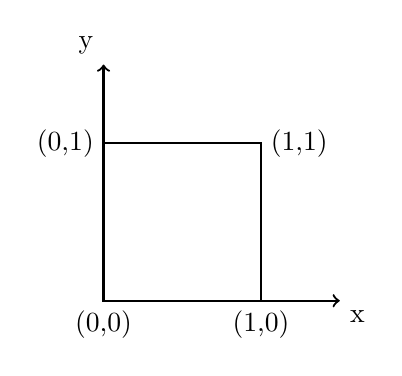
\begin{tikzpicture}[scale=2]
			% Draw grid and axes
			\draw[step=1cm,gray,very thin] (0,0) grid (1,1);
			\draw[thick,->] (0,0) -- (1.5,0) node[anchor=north west] {x};
			\draw[thick,->] (0,0) -- (0,1.5) node[anchor=south east] {y};

			% Draw square
			\draw[thick] (0,0) -- (0,1) -- (1,1) -- (1,0) -- cycle;

			% Label points
			\node[anchor=north] at (0,0) {(0,0)};
			\node[anchor=north] at (1,0) {(1,0)};
			\node[anchor=east] at (0,1) {(0,1)};
			\node[anchor=west] at (1,1) {(1,1)};
		\end{tikzpicture}
	\end{figure}
\end{frame}
\begin{frame}[fragile]{Koordinatengrafik}
	\begin{lstlisting}[style=python]
import turtle as t

def star():
    for _ in range(6):
        t.forward(30)
        t.right(140)
        t.forward(30)
        t.left(80)

t.clear("blue")
t.fillcolor("yellow")
t.setpos(20,100)
t.begin_fill()
star()
t.end_fill()
\end{lstlisting}
\end{frame}
%
\begin{frame}[fragile]{Zufallszahlen}
	\begin{lstlisting}[numbers=none,style=python, basicstyle=\ttfamily\scriptsize]
import turtle as t
import random

def star():
    for _ in range(6):
        t.forward(10)
        t.right(140)
        t.forward(10)
        t.left(80)

t.clear("blue")
t.fillcolor("yellow")
for _ in range(50):
    x = random.randint (-270, 270)
    y = random.randint (-270, 270)
    t.setpos(x,y)
    t.begin_fill()
    star()
    t.end_fill()
\end{lstlisting}
\end{frame}
\begin{frame}{Turtle-Dokumentation \emoji{turtle}}
	$\rightarrow$ Ausführliche Dokumentation: \href{https://jython.ch/index.php?inhalt_links=navigation.inc.php&inhalt_mitte=turtle/turtledoc.html}{Link}
	\begin{mycaution}
		Nicht alle Befehle funktionieren! Immer zuerst testen auf \url{https://webtigerpython.ethz.ch} ($\rightarrow$ Prüfungs-Plattform!).

	\end{mycaution}
\end{frame}

\begin{frame}{Aufträge}
	\begin{enumerate}
		\item \emoji{switzerland} Zeichnen Sie ein Schweizer Kreuz (\textbf{Tipp}: zuerst ohne Farben, danach farbig).
		\item Zeichnen Sie die Flagge vom Kanton Zürich (quadratisch). 
\includegraphics[width=0.1\linewidth]{Grundlagen_Info/00_Programmieren/Figures/Flag_of_Canton_of_Zürich}\definecolor{zhblue}{RGB}{0,112,180}
		      \textcolor{zhblue}{(Farbe ``Züri-Blau'': 0, 112, 180)}
		\item Sie ein horizontal dreigeteiltes Flaggen (wie etwa das von Frankreich \emoji{flag-france} oder Italien \emoji{flag-italy}).
		\item \textbf{Challenge}: Dasselbe wie Aufgabe 3, aber die Breite der Farben soll zufällig sein (bei jeder Ausführung anders).
		\item \textbf{Challenge}: Dasselbe wie Aufgabe 3, aber die Breite der Farben sowie die Farben sollen zufällig sein (bei jeder Ausführung anders).
	\end{enumerate}

\end{frame}
